\documentclass{article}
\usepackage{fixltx2e}
\usepackage[utf8]{inputenc}
\usepackage{graphicx}
\usepackage{sidecap}
\usepackage{fancyhdr}
\usepackage[margin=1.5in]{geometry}
\usepackage{amssymb,amsmath}
\usepackage[euler]{textgreek}
\usepackage[swedish]{babel}


\setlength{\headheight}{21pt}

\begin{document}

% Titelsida -----------------------------
\begin{titlepage}
\begin{center}

% Upper part of the page. The '~' is needed because \\
% only works if a paragraph has started.

\textsc{\LARGE Link{\"o}pings Universitet}\\[1.5cm]


% Title
{ \huge \bfseries Modellbaserad reglering av dubbeltankar \\[0.4cm] }

% Author and supervisor
\large
\emph{Av:}\\
Hans-Filip \textsc{Elo} och Niklas \textsc{Ericson}

\vfill

% Bottom of the page
{\large \today}

\end{center}

% Slut på titelsida. ---------------------

% Innehåll ------------------------------
\newpage
\thispagestyle{empty}
\tableofcontents
\listoffigures
\listoftables

\end{titlepage}
%header ---------------------------------
\pagestyle{fancy}

\fancyhead{} % clear all header fields
\fancyhead[L]{TSRT12\slshape}
\fancyhead[R]{\today \slshape}

\fancyfoot{} % clear all footer fields
\fancyfoot[L,R]{\thepage}
\fancyfoot[L]{Modellbaserad reglering av dubbeltankar}

%slut på header ---------------------------------


\section{Inledning}
En överföringsfunktions egenskaper så som stigtid, översläng och felmarginal går att påverka genom att multiplicera funktionen med en deriverande, F\textsubscript{lead}, och en integrerande, F\textsubscript{lag}, funktion. En laboration med ett dubbeltanksystem har genomförts för att applicera teorin i verkligheten.

\section{Syfte}
Syftet med laborationen var att färdigställa en överföringsfunktion för systemet med dubbeltankar och sedan reglera systemet så det uppnår givna specifikationskrav. 

\section{Metod}

En överföringsfunktion för systemet var given enligt nedan. 

\begin{equation}
G\textsubscript{dubbel}(s) = \frac{K_{enkel1}}{sT+1} * \frac{K_{enkel2}}{sT+1} = \frac{K\textsubscript{dubbel}}{(sT+1)^2}
\end{equation}
\\
Där {\itshape T}, K\textsubscript{enkel1} och K\textsubscript{enkel2} är konstanter. K\textsubscript{dubbel} är produkten av K\textsubscript{enkel1} och K\textsubscript{enkel2}. 
\\
\\
Laborationen bestod av 2 delar. Första delen bestod av att ta fram två okända konstanter, {\itshape T} och {\itshape K}\textsubscript{dubbel}, medan den andra delen bestod i att ta fram en F\textsubscript{lead} och en F\textsubscript{lag} funktion som gav önskade egenskaper på systemet. 
\\

\subsection{Framtagning av konstanter}
Konstanterna kan bägge två lösas ut ur givet stegsvar för systemet, men resulterar då i en ekvation med två okända. Vi kommer alltså att behöva göra mätningar för att approximera aktuella konstanter. 

\subsubsection{Att ta fram {\itshape T}}
Konstanten {\itshape T} går att finna genom att skicka in ett steg i systemet och mäta stigtiden för utsignalen till 63\% av steget i utsignalen. Detta fås ur överföringsfunktionen för en av tankarna och laplacetransformen av ett enhetssteg (1/s) enligt nedan. 

\begin{equation}
\delta_{u}(s) = \frac{C * K_{enkel1}}{sT+1}{(sT+1)s}
\end{equation}
\\
Där \textdelta\textsubscript{u}(s) är skillnaden i utsignalen (vattennivå) och C är höjden på steget in. Inverstransformerar man sedan detta och sätter \textdelta\textsubscript{u}(t) = 0,63K\textsubscript{enkel}C. Löser man sedan ut {\itshape T} detta får man enligt ekvation nedan. 

\begin{equation}
T = \frac{-t}{ln{0,37}} \approx t
\end{equation}
\\
Där tiden t är tiden då utsignalen nått upp till 0,63\% av differensen mellan stationär vattennivån innan och efter stegskillnad getts i insignal. Man behöver alltså göra mätningar för att finna T. 
\\

\subsubsection{Att ta fram K\textsubscript{dubbel}}

\subsection{Framtagning av T och K\textsubscript{dubbel}}
I förberedelseuppgifterna till laboration visades att tidskonstanten, {\itshape T} fås av den tid det tar för stegsvaret att nå 63\% av slutvärdet. Ekvationen för ett första ordningens system ser ut som i (1) nedan. Väl i laborationen sattes en arbetspunkt på 10cm och utifrån denna applicerades en spänningsökning som motsvarar ett enhetssteg. När nivån hade nått 10,63 lästes tidskonstanten, {\itshape T} ut som den tid det tagit från att steget applicerats. 

\begin{equation}
\delta_{h1}(t)= c*K_{enkel}*(1-e^{\frac{-t}{T}})
\end{equation}
\\

\subsection{Materiel}

\subsection{Specifikationer}

\section{Resultat}
Mätningen utfördes 3 gånger med samma steg från samma arbetspunkt. Resultatet av mätningarna ges i tabell 1 nedan. Arbetspunkten var under mätningarna 10cm (1,23V). Enhetssteget ökade nivån genom att spänningsnivån höjdes till 1,28V. 

\begin{table}[ht] 
\centering 
\begin{tabular}{c c} 
Försök & T \\ [0.5ex] % inserts table heading
\hline
1 & 17 \\
2 & 18 \\
3 & 20 \\

\end{tabular} 
\caption{Tabell över mätvärden på tidskonstanten.}

\end{table}
~\\ %weird ass quickfix
Medelvärdet på T räknades ut till T=18.4 och därmed var tidskonstanten bestämd. 
Bestämningen av K\textsubscript{dubbel} gick till på liknande vis. En ekvation söktes för K\textsubscript{dubbel} och vid stationaritet kan slutvärdessatsen användas se ekvation 2. 
 
\begin{equation}
\lim\limits_{t \to \infty}y(t) = \lim\limits_{s \to 0}sY(s)
\end{equation}
\pagebreak
\\
Utsignalen för dubbeltankssystemet fås alltså vid stationaritet enligt ekvation 3 där u är den spänning som applicerats för att utföra steget. 
\begin{equation}
\delta_{h1}(t)=\lim\limits_{s \to 0}s*\frac{K_{dubbel}}{(1+s)^2}*\frac{u}{s}=uK_{dubbel}
\end{equation}
\\
Mätningen utfördes även här tre gånger men denna gång var steget lite olika från gång till gång. Resultatet av mätningarna ges i tabell 2 nedan. Arbetspunkten var under mätningarna 10cm (1,09V). Enhetssteget ökade nivån genom att spänningsnivån höjdes till 1,14V dvs med u=0,05V. 

\begin{table}[ht] 
\centering 
\begin{tabular}{c c} 
Försök & $\delta_{h2}$ \\ [0.5ex] % inserts table heading
\hline
1 & 1,46 \\
2 & 1,07 \\
3 & 1,36 \\

\end{tabular} 
\caption{Tabell över mätvärden på $\delta_{h2}$.}
\end{table}
~\\ %weird ass quickfix
Medelvärdet räknades ut till $\delta_{h2}=1,3$ vilket dividerat på u=0,05V ger K\textsubscript{dubbel}=25,9


\subsection{Förändring av systemets egenskaper}


\begin{figure}[ht!]
\centering
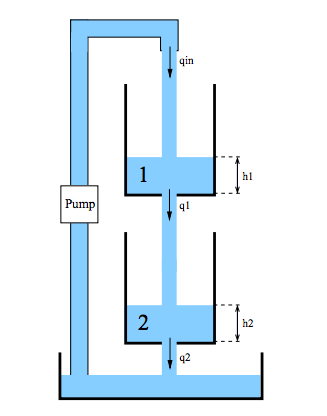
\includegraphics[width=70mm]{System.png}
\caption{Visualisering av labuppkopplingen}
\label{overflow}
\end{figure}

\begin{figure}[ht!]
\centering
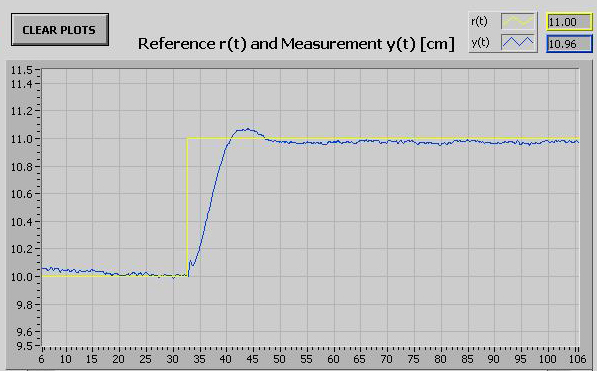
\includegraphics[width=90mm]{Test1_cut.jpg}
\caption{Stegsvaret efter kompensering med F\textsubscript{lead} och F\textsubscript{lag}.}
\label{overflow}
\end{figure}


\section{Slutsats}

\end{document}